\chapter{Metodologia\label{cap:metodologia}}

	A metodologia possuiu dois pilares: sólida base em Algoritmos Genéticos e desenvolvimento de um \emph{software} confiável para execução do modelo. Ambos são apresentados nas seções seguintes.

%========================================================
\section{Algoritmos Genéticos}\label{seq:medologia_ga}
%========================================================
	
	Iniciei os estudos em Algoritmos Genéticos pelos livros \cite{Mitchell98} e \cite{Linden2008} e, antes de partir para o trabalho da dissertação em si, ataquei três problemas completamente distintos.
	
	O primeiro foi o ONEMAX \cite{onemaxNaGPU}, desenvolvido ``do zero'', em Linguagem C. Considerado o \emph{hello world} do GA, tem representação cromossomial binária, o \emph{fitness} é a soma dos \emph{bits} de cada indivíduo e o objetivo é obter um indivíduo com o maior número de '1' possível. Com ele pude estudar os parâmetros de um GA simples, como número de indivíduos e a probabilidade de \emph{crossover}, e verificar a influência de cada um na qualidade da solução, convergência, desempenho, evolução do \emph{fitness} etc. Uma versão paralelizada em CUDA foi apresentada em evento de computação de alto desempenho \cite{ERAD12} e é discutida na seção \ref{sec:oneMaxNaGPU}.
	
	\begin{figure}[htbp]
		\centering
			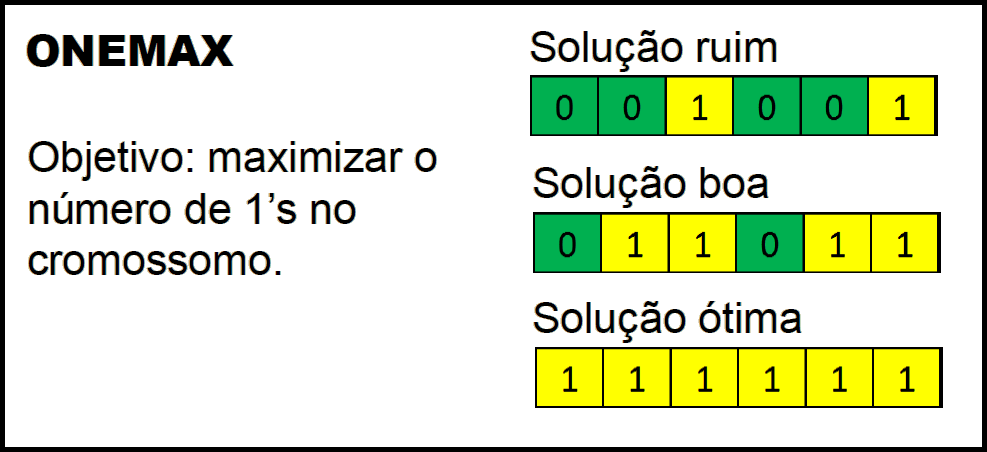
\includegraphics[width=0.60\textwidth]{figs/resultados/onemax/onemax_objetivo.png}
		\caption{ONEMAX: representação cromossomial, \emph{fitness} e objetivo.}
		\label{fig:onemax_objetivo_metodologia}
	\end{figure}
	
	Tendo a estrutura básica do ONEMAX, o próximo passo foi tentar fazer um modelo. Abordei o Problema das Oito Rainhas, que consiste em posicionar oito rainhas em um tabuleiro de xadrez de modo que não se ataquem. Sem nenhuma referência externa, propus um modelo de GA que conseguiu chegar em algumas soluções \cite{qualificacao_adriano}. Uma delas está na figura \ref{fig:OitoRainhasSolucao}.
	
	\begin{figure}[htbp]
		\centering
			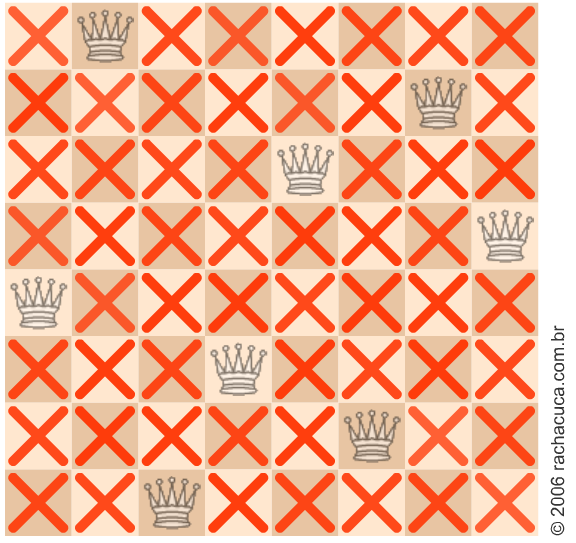
\includegraphics[width=0.30\textwidth]{figs/materiais_metodo/ga/OitoRainhasSolucao.png}
		\caption{Uma solução para o Problema das 8 Rainhas.}
		\label{fig:OitoRainhasSolucao}
	\end{figure}
	
	Tratando o tabuleiro de xadrez como um plano cartesiano, a representação cromossomial era um \emph{string} com os oito pares de coordenadas $(x,y)$. Cada coordenada gerava uma matriz característica de 0's e 1's que, quando somadas, resultava em uma matriz com a informação da quantidade $c$ de ataques que cada rainha sofreu. O objetivo, portanto, era encontrar um indivíduo que levasse a $c = 0$. A função de avaliação foi definida como $f = 1/(1 + c)$.
	
	Criar um modelo para o Oito Rainhas foi importante para o entendimento do elo entre um GA e o problema a ser resolvido. Essa ligação encontra-se na representação cromossomial e na função de avaliação. Defini ambas de maneira adequada, mas a representação cromossomial apresentou um problema: nada impede de haver pontos $(x,y)$ repetidos no cromossomo. Em outras palavras, ela permite que duas rainhas sejam colocadas na mesma posição do tabulareiro, o que é proibido no xadrez. 
	
	Por fim, utilizei GA na criação de um robô, chamado \emph{Genético}, para ser testado contra os campeões do torneio de Robocode da Faculdade de Tecnologia da Unicamp\footnote{\texttt{http://torneiorobocode.orgfree.com/torneio-ft.php}}. Robocode é um jogo\footnote{\texttt{http://robocode.sourceforge.net/}}, cujo objetivo é programar um tanque de guerra robô para competir contra outros robôs em uma arena de batalha. Ele começou como um projeto pessoal no ano 2000 e depois foi incorporado pela IBM\footnote{\texttt{http://robocode.sourceforge.net/docs/ReadMe.html}}. Atualmente é um projeto de código aberto.
	
	\begin{figure}[htbp]
		\centering
			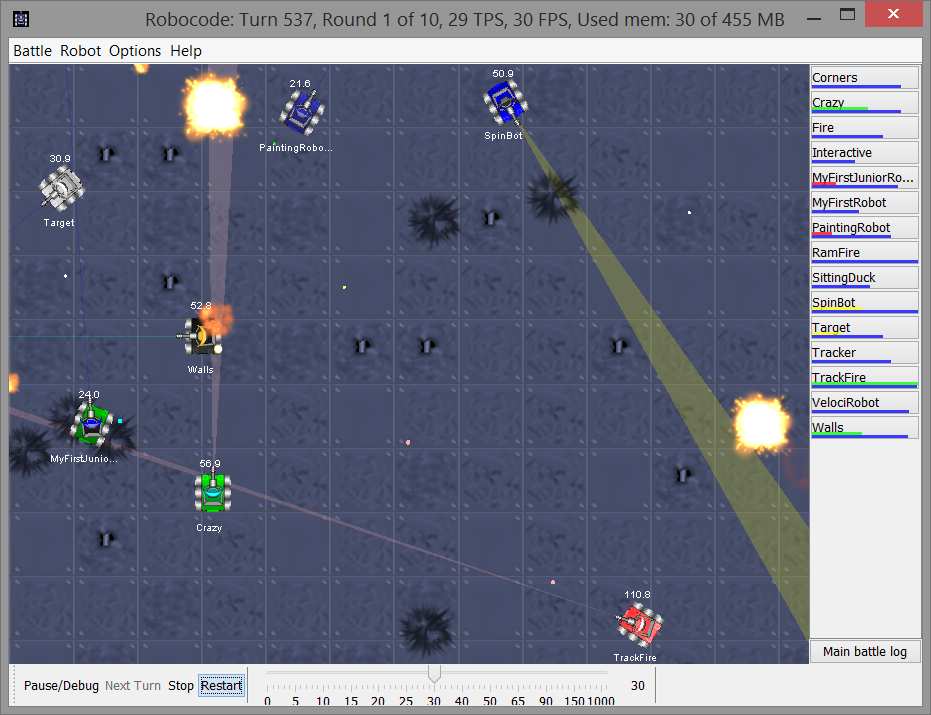
\includegraphics[width=0.50\textwidth]{figs/materiais_metodo/ga/Robocode_Battle_Field.PNG}
		\caption{Arena de batalha do Robocode.}
		\label{fig:Robocode}
	\end{figure}
	
	Baseei-me no artigo \cite{robocodeGA}, publicado em um congresso de computação evolutiva da IEEE. As primeiras versões do \emph{Genético} não travaram boas batalhas. Alterei o \emph{fitness} e o processo de treinamento. Na versão final ele foi capaz de vencer os robôs que ficaram em primeiro e terceiro lugares no torneio daquele ano (o segundo lugar não estava disponível para \emph{download}). O \emph{Genético} vencia, inclusive, contra os dois simultaneamente \cite{robocodeGA_adriano}.
	

%========================================================
\section{\emph{Software}}
%========================================================

	O \emph{software} utilizado foi totalmente desenvolvido por mim, e há razões metodológicas que justificam essa escolha. Obtive bons resultados criando os próprios programas nos estudos iniciais de GA. Eles foram fundamentais para que eu soubesse exatamente o que estava acontecendo durante a execução. Quis ter esse controle total também sobre o programa que executaria o GA proposto para esta dissertação. Ele foi escrito em Linguagem C, utilizando apenas quatro bibliotecas padrão: \texttt{stdio.h}, \texttt{stdlib.h}, \texttt{time.h} e \texttt{math.h}. Portanto, é totalmente portável para os sistemas operacionais que possuem um compilador C$++$. Além disso, C é a linguagem nativa da arquitetura CUDA, o que facilitará sua paralelização.
	
	Tive muito cuidado com a confiabilidade dos resultados. Quando opta-se por não gerá-la automaticamente, a \emph{semente} dos números pseudo-aleatórios é um dos parâmetros de entrada. Duas execuções com os mesmos parâmetros, incluindo a semente, levam a exatamente os mesmos resultados. Por isso nas tabelas e gráficos deixei explícito seu valor. Os gráficos encontrados em \cite{metodo2004} e \cite{metodo2011} referem-se ao maior \emph{fitness} (e $\rho$ associado) de cada geração. O programa gera essa informação, mas também exibe as médias dessas variáveis. De acordo com \cite{Mitchell98}, uma teoria geral para entender e prever o comportamento dos GAs seria análoga à Mecânica Estatística na Física. Ao contrário de lidar com grande número de componentes do sistema, como a composição genética exata de cada população, tal abordagem trabalha com uma estatística mais ``macroscópica'', como o \emph{fitness} médio da população. Portanto, tanto os critérios de parada do programa quanto a minha análise foram baseadas em médias.
	
%---------------------------------------------------
\subsection{Como utilizar o programa}
%---------------------------------------------------	
	
	Para utilizar o \emph{software} basta baixar o código e compilar o arquivo \texttt{Serial\_novo.c} (será necessário alterar o diretório no \emph{include} das bibliotecas que desenvolvi). O código está disponível na internet para qualquer um utilizar, testar e, inclusive, melhorar\footnote{\texttt{https://github.com/prietoab/msc\_code}}. Caso isso aconteça, peço apenas que cite esta dissertação.
	
		A execução dá-se via linha de comando passando os parâmetros necessários. Porém, como são muitos parâmetros, é aconselhável a utilização de um arquivo de \emph{script}. Assim é possível criar processos de varredura para variar os parâmetros desejados ou repetir várias execuções. Fiz isso para automatizar o estudo e ter dados suficientes para análise. Na figura \ref{fig:script_windows} há um exemplo de \emph{script} Windows para fazer execuções variando o número de genes.
			
		\begin{figure}[htbp]
			\centering
				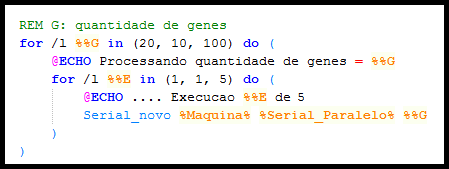
\includegraphics{figs/materiais_metodo/software/script_windows.png}
			\caption{Exemplo de \emph{script} Windows para fazer execuções variando o número de genes.}
			\label{fig:script_windows}
		\end{figure}

	Não é necessário ter uma matriz para execução. Por meio do parâmetro \emph{Tamanho do cromossomo} (seção \ref{sec:listaParametros}) o programa gera automaticamente uma matriz de Coope \cite{Coope1977}, definida na equação \ref{eq:MatrizCoope}. Essa matriz foi utilizada nos testes de \cite{metodo2011}.
	
	\begin{equation}\label{eq:MatrizCoope}
		\begin{array}{ccl}
			H(i,i) = 2i - 1 			& , & i = 1, 2, ..., n. \\
														&		&		\\
			H(i,j) = H(j,i) = 1		& , & i \neq j; \\
														&		& i = 1, 2, ..., n; \\
														&		& j = 1, 2, ..., n.
		\end{array}
	\end{equation}
	
%---------------------------------------------------
\subsection{Informações de saída}
%---------------------------------------------------	
		
Há cinco grupos de informações na saída do programa. Usados em conjunto dão um panorama do algoritmo genético. Para apenas um deles (Estatística) um arquivo texto é gerado automaticamente. Os outros são exibidos na tela. Para alterar a saída padrão para um arquivo texto, é necessário utilizar o caractere de redirecionamento da saída padrão. No Windows, Linux e Unix esse caractere é o ``>''. No Linux, por exemplo, o comando ``\texttt{ls > dirs.txt}'' lista o conteúdo do diretório atual e armazena no arquivo \texttt{dirs.txt}.

\begin{enumerate}

	\item \textbf{Cabeçalho}
	
		Contém todos os parâmetros de execução recebidos na linha de comando. Impresso na tela.
	
	\item \textbf{Comportamento do \emph{fitness}}
	
		Imprime na tela, para cada geração, além de alguns parâmetros de execução, as seguintes informações: 
		
		\begin{itemize}
			\item $\rho$ mínimo
			\item $\rho$ médio (<$\rho$>)
			\item \emph{fitness} médio (<\emph{fitness}>)
			\item Maior \emph{fitness}
			\item $\rho$ associado ao maior \emph{fitness}
			\item <$|\nabla \rho|^2$>
			\item Posição do melhor indivíduo
		\end{itemize}

	\item \textbf{Tempos de processamento}
	
		Imprime na tela uma estimativa para o tempo de processamento (em \emph{clocks}) para cada operador. Se o programa foi executado por 200 gerações, haverá 200 tempos de processamento para o \emph{fitness}, seleção, \emph{crossover} e mutação.
		
	\item \textbf{Geração final}
	
				Impressão de todos os indivíduos da última geração. 
	
	\item \textbf{Estatística}
	
				A cada execução é criado (ou atualizado caso já exista) um arquivo chamado \texttt{estatistica.txt}. Nele, além de todos os parâmetros, há informações relacionadas à geração que atingiu algum critério de parada. Por exemplo, além do próprio número da última geração, há o \emph{fitness} médio, o maior \emph{fitness}, o $\rho$ associado ao maior \emph{fitness}, o $\rho$ médio e o tempo total de processamento do programa.
	
\end{enumerate}
	
%---------------------------------------------------
\subsection{Lista dos arquivos fonte}
%---------------------------------------------------
	
	O programa é pequeno ($\approx$ 2500 linhas), e está distribuído em seis arquivos, um principal e cinco bibliotecas:
	
	\begin{itemize}
		\item \textbf{Serial\_novo.c}
		
		Arquivo principal. Contém o fluxo do GA (figura \ref{fig:fluxo}).
		
		\item \textbf{Estruturas.h}
		
		Contém as estruturas de dados e uma função que retorna automaticamente o parâmetro $\lambda$ do \emph{fitness} (seção \ref{sec:eq_lambda}).
		
		\item \textbf{Algebra\_Linear\_serial.h}
		
		Mutiplicação e subtração de matrizes.
		
		\item \textbf{Estatistica.h}
		
		Média, variância e desvios do Quociente de Rayleigh.
		
		\item \textbf{Auxiliares\_serial.h}
		
		Números pseudo-aleatórios, alocação de memória para indivíduos na população.
		
		\item \textbf{GA\_Serial.h}
		
		Contém as funções do Algoritmo Genético. A maioria do código está nessa biblioteca.	
		
	\end{itemize}
					
%---------------------------------------------------
\subsection{Lista dos parâmetros de execução}
\label{sec:listaParametros}
%---------------------------------------------------
	\begin{enumerate}
		\item \textbf{Código da máquina}.
		
				Número inteiro, utilizado para identificar o computador que o programa foi executado. Útil para comparar as execuções em computadores diferentes. Por exemplo, se há quatro computadores A, B, C e D, é possível classificá-los como A = 0, B = 1, C = 2, D = 3.
				
		\item \textbf{Serial ou Paralelo}?
		
				Número inteiro. Determina se a execução será serial (= 0) ou paralela (= 1). A atual versão permite apenas execução serial. Portanto, esse parâmetro pode ser fixado em zero.
				
		\item \textbf{Tamanho do cromossomo (ordem da matriz de Coope)}.
		
				Número inteiro. Determina a ordem da matriz de Coope. Inserir 200 nesse parâmetro gera uma matriz de Coope de tamanho 200 x 200.
			
		\item \textbf{Quantidade máxima de gerações}.
		
				Número inteiro. Um dos critérios de parada. Para evitar que o programa entre em um \emph{loop} infinito caso não haja convergência para uma solução. Se definida como 100, o programa executará, no máximo, 100 iterações de Avaliação, Seleção, \emph{Crossover} e Mutação.
		
		\item \textbf{Quantidade de indivíduos na população}.
		
		Número inteiro. Determina a quantidade de indivíduos em cada população.
		
		\item \textbf{Tipo do Fitness}.
		
		Número inteiro. O programa pode trabalhar com cinco tipos de \emph{fitness}. Dois deles são os apresentados na seção \ref{sec:fitness_metodo}. Qualquer código diferente dos apresentados abaixo faz com que o \emph{fitness} seja definido como $f = -1$.
		
			\begin{itemize}
				\item Tipo 0 \cite{metodo2011}:
				
					\begin{equation}
					f = e^{-\lambda(\rho - E_L)^2}
					\end{equation}
				
				\item Tipo 1 \cite{metodo2004}:
				
					\begin{equation}
					f = e^{-\lambda |\nabla \rho|^2}
					\end{equation}
					
				\item Tipo 2:
				
					\begin{equation}
					f = e^{-\lambda [(\rho - E_L)^2 + |\nabla \rho|^2]}
					\end{equation}
					
				\item Tipo 3:
				
					\begin{equation}
					f = e^{-\lambda |\nabla \rho|}
					\end{equation}
		
			\item Tipo 4:
				
					\begin{equation}
					f = e^{-\lambda [(\rho - E_L)^2 + |\nabla \rho|]}
					\end{equation}
			\end{itemize}
			
		\item \textbf{Tipo do Fitness Paralelo}.
		
				Número inteiro. A atual versão permite apenas execução serial. Portanto, esse parâmetro pode ser fixado em zero.
		
		\item \textbf{Tamanho do Torneio}
		
			Número inteiro. Define a quantidade de indivíduos selecionados para o torneio na Seleção.
		
		\item \textbf{Probabilidade do \emph{Crossover}}.
		
			Número real. Define, em porcentagem, a probabilidade de \emph{Crossover}. Exemplo: 80.5 = 80,5\%.
		
		\item \textbf{Quantidade de Pontos de Corte}.
		
			Número inteiro. Na versão atual a quantidade de pontos de corte foi fixada em dois conforme o operador de \emph{crossover} definido na seção \ref{sec:crossover_utilizado}. Pode ser mantido como zero.
		
		\item \textbf{Probabilidade de Mutação}.
		
		Número real. Define, em porcentagem, a probabilidade de mutação. Exemplo: 12.7 = 12,7\%.
		
		\item \textbf{Intensidade da Mutação - $\Delta$}.
		
			Número real. Define o parâmetro $\Delta$ utilizado no \emph{crossover}. É dividido por dez. Exemplo: $1.2$ no parâmetro $\rightarrow 0,12$ no $\Delta$.
		
		\item \textbf{Valor para $\lambda$}.
		
		Número real. Define o valor do parâmetro $\lambda$ do \emph{fitness}. Se for configurado como $-1$, um valor adequado para $\lambda$ é gerado automaticamente.
		
		\item \textbf{Valor para $E_L$}.
		
		Número real. Define um limite inferior para o autovalor mínimo ($E_0$) nos \emph{fitness} de tipo 0, 2 e 4. 
		
		\item \textbf{Precisão - $\xi$}.
		
		Número real. Define a precisão dos critérios de parada. O programa termina se a variável alvo é menor ou igual a $\xi$. Depende do tipo de \emph{fitness}.
		
		Condições de parada em função do \emph{fitness} ($<x>$ significa valor médio de $x$):
				
		\begin{itemize}
			\item Fitness tipos 0, 2 e 4:
						
			\begin{equation}\label{eq:criterioParada024}
				\begin{array}{ccll}
				<|\nabla \rho|> & \leq & \xi & \mbox{  ou} \\
				| <\rho> - E_L | & \leq & \xi &
				\end{array}
			\end{equation}
			
			
			\item Fitness tipos 1 e 3:
			
			\begin{equation}\label{eq:criterioParada13}
				\begin{array}{ccll}
					<|\nabla \rho|> & \leq & \xi &
				\end{array}
			\end{equation}
			
		\end{itemize}
		
		\item \textbf{Imprime comportamento do \emph{Fitness}}?
		
		Se configurado como Verdadeiro (1), imprime na saída padrão as variáveis de interesse para estudar o comportamento do \emph{fitness}. 
		
			0: \emph{Falso}. Não imprime.
			
			1: \emph{Verdadeiro}. Imprime.
		
		\item \textbf{Imprime tempos de execução}?
		
			Número inteiro. Se configurado como Verdadeiro (1), imprime na saída padrão os tempos estimados de execução (em \emph{clocks} do processador) das funções e operadores.
			
			
			0: \emph{Falso}. Não imprime.
			
			1: \emph{Verdadeiro}. Imprime.
			
		
		\item \textbf{Gera nova semente para números pseudo-aleatrórios}?
		
		Número inteiro. Se configurado como Verdadeiro (1), o programa cria uma nova semente para os números pseudo-aleatórios. Caso contrário, a semente definida no próximo parâmetro é utilizada.
		
		0: \emph{Falso}. Utiliza semente definida no parâmetro \emph{Semente}.
		
		1: \emph{Verdadeiro}. Cria uma nova semente. O parâmetro \emph{Semente} é ignorado.
		
		\item \textbf{Semente dos números pseudo-aleatrórios}.
		
		Número inteiro. Define a semente dos números pseudo-aleatórios. Depende do parâmetro anterior.
		
		\item \textbf{Tipo do cálculo de $\nabla \rho$}.
		
		Deve ser configurado como 1.
		
		Nas versões iniciais $\nabla \rho$ era calculado literalmente como na equação \ref{eq:grad_rho_metodo}, exigindo o uso de uma matriz identidade ($I$) da ordem do Hamiltoniano. A equação foi reescrita internamente de modo que $I$ não fosse necessária, liberando memória e fazendo menos operações. Usar ou não $I$ leva aos mesmos resultados.
		
		0: Utiliza matriz identidade.
		
		1: Não utiliza matriz identidade (libera memória e faz menos operações).
		
	\end{enumerate}
	
%---------------------------------------------------
\subsection{Estruturas de Dados}
%---------------------------------------------------	

	Cinco estruturas de dados formam a base do programa. Elas estão definidas no arquivo Estruturas.h.
	
%----
\subsubsection{parametrosPrograma}
%----

	Responsável por armazenar os parâmetros de execução, descritos na seção \ref{sec:listaParametros}.
	

\vspace{1 cm}	
\begin{lstlisting}
struct parametrosPrograma {
  unsigned short int parmMaquina;
  unsigned short int parmSerial_ou_Paralelo;
  unsigned short int parmQtdeGenes;
  unsigned long int parmQtdeMaxGeracoes;
  unsigned short int parmQtdeIndividuos;
  char parmTipoFitnessEquacao;
  char parmTipoFitnessParalelo;
  char parmTipoCalculoGradRho;
  char parmTamanhoTorneio;
  double parmProbCrossOver;
  unsigned short int parmQtdePontosCorte;
  double parmProbMutacao;
  double parmIntensidadeMutacao;
  double parmLambda;
  double parmRhoMinimo;
  double parmTolerancia;
  unsigned short int parmFlagImprimeComportamentoFitness;
  unsigned short int parmFlagImprimeTempo;
  unsigned short int parmFlagNovaSemente;
  unsigned long int parmSemente;
};
\end{lstlisting}
\vspace{1 cm}

%----
\subsubsection{parametros\_Metodo}
%----

	Armazena os parâmetros do \emph{fitness}, $\lambda$ e $E_0$.


\vspace{1 cm}	
\begin{lstlisting}
struct parametros_Metodo {
  double lambda;
  double rho_minimo;
};
\end{lstlisting}
\vspace{1 cm}

%----
\subsubsection{parametros}
%----
	
	Parâmetros do algoritmo genético.
	

\vspace{1 cm}	
\begin{lstlisting}
struct parametros {
  unsigned short int numGenes;
  unsigned short int numIndividuos;
  double probCrossOver;
  double probMutacao;
  double intensidadeMutacao;
  char tamanho_torneio;
  unsigned short int qtde_Pontos_de_Corte;
};
\end{lstlisting}
\vspace{1 cm}

%----
\subsubsection{individual}
%----

	Essa estrutura representa o cromossomo, o indivíduo, do algoritmo genético.
	
	\textbf{\texttt{cociente\_Rayleigh}}: $\rho_i$.
	
  \textbf{\texttt{grad\_elevado\_ao\_quadrado}}: $|\nabla \rho_i|^2$.
	
  \textbf{\texttt{rho\_menos\_rho0\_ao\_quadrado}}: $(\rho_i - E_0)^2$.
	
  \textbf{\texttt{Numerador}}: Recebe o retorno do cálculo $C_i^\dagger H C_i$, utilizado na equação \ref{eq:rho-GA}, seção \ref{sec:fitness_metodo}.
  
	\textbf{\texttt{CtC}}: Recebe o produto escalar de $C{_i}^{\dag}C_i$, utilizado no cálculo da equação \ref{eq:rho-GA}, seção \ref{sec:fitness_metodo}.
  
	\textbf{\texttt{inverso\_de\_CtC}}: $(C_i^{\dag}C_i)^{-1}$.
  
	\textbf{\texttt{fitness}}: recebe o valor do \emph{fitness} do indivíduo, independente do tipo.
  
	\textbf{\texttt{pontos\_de\_corte(2)}}: Vetor de tamanho fixo, cuja função é armazenar as duas posições que determinarão a posição inicial e final do \emph{crossover}.
  
	\textbf{\texttt{*gene}}: Ponteiro de memória para um vetor que armazenará os valores dos genes do cromossomo. O tamanho desse vetor é dado pelo parâmetro \texttt{numGenes} da estrutura \texttt{parametros}.
  
	\textbf{\texttt{*gradRho}}: Ponteiro de memória para um vetor que armazenará os valores dos componentes do vetor $\nabla\rho_i$. O tamanho desse vetor é dado pelo parâmetro \texttt{numGenes} da estrutura \texttt{parametros}.
	

\vspace{1 cm}	
\begin{lstlisting}
struct individual {
  double cociente_Rayleigh;
  double grad_elevado_ao_quadrado;
  double rho_menos_rho0_ao_quadrado;
  double Numerador;
  double CtC;
  double inverso_de_CtC;
  double fitness;
  unsigned short int pontos_de_corte[2];
  double *gene;
  double *gradRho;
};
\end{lstlisting}
\vspace{1 cm}

%----
\subsubsection{generation}
%----

		A estrutura \texttt{\textbf{generation}} representa a população dos indivíduos em um dado instante de tempo. O programa possui apenas duas, utilizadas alternadamente a cada aplicação de um operador genético. Por exemplo, \textbf{Seleção}(\texttt{geracao0}) $\rightarrow$ \texttt{geracao1}, e em seguida Crossover(\texttt{geracao1}) $\rightarrow$ \texttt{geracao0}.

	\textbf{\texttt{sumFitness}}: Soma do \emph{fitness} de todos os indivíduos da população. Utilizada para obter o \emph{fitness} médio $<f>$.
	
  \textbf{\texttt{FitnessMedio}}: $<f>$.
	
	\textbf{\texttt{sumRho}}: Soma do $\rho$ de todos os indivíduos da população. Utilizada para obter o quociente de Rayleigh médio $<\rho>$.
	
  \textbf{\texttt{rhoMedio}}: $<\rho>$.
	
  \textbf{\texttt{difRho}}: $<\rho> - E_L$
	
  \textbf{\texttt{sumGradRho}}: Soma de todos os $|\nabla \rho_i|$. Utilizada para obter $<|\nabla \rho|>$.
	
  \textbf{\texttt{gradRhoMedio}}: $<|\nabla \rho|>$
	
  \textbf{\texttt{Maior\_fitness}}: Maior \emph{fitness} da população.
	
  \textbf{\texttt{Melhor\_cociente\_Rayleigh}}: $\rho$ associado ao maior \emph{fitness} da população.
	
	\textbf{\texttt{idxMelhorIndividuo}}: Posição do melhor indivíduo no vetor de indivíduos. Por exemplo, se há 10 cromossomos na população, seu valor pode ser 0, 1, 2, ..., 9.
	
  \textbf{\texttt{*individuo}}: Ponteiro de memória para o vetor que contém os indivíduos da população.
	

\vspace{1 cm}
\begin{lstlisting}
struct generation {
  double sumFitness;
  double FitnessMedio;
  double rhoMedio;
  double sumRho;
  double difRho;
  double sumGradRho;
  double gradRhoMedio;
  double Maior_fitness;
  double Melhor_cociente_Rayleigh;
  unsigned short int idxMelhorIndividuo;
  struct individual *individuo; // alocar constNumIndividuos;
};
\end{lstlisting}
\vspace{1 cm}

%---------------------------------------------------
\subsection{População inicial}
%---------------------------------------------------

	Está no arquivo \textbf{\texttt{GA\_serial.h}}.
	
	O objetivo da \texttt{GeraPopulacaoInicial\_serial} é criar os valores aleatórios para os genes de todos os indivíduos. As outras variáveis da geração e dos indivíduos são apenas inicializadas. Ela como parâmetros dois ponteiros (linhas 3 e 4), um para a população e outro para os parâmetros do GA.
	
	O \emph{loop} principal varre todos os indivíduos da população, e o laço interno caminha pelos genes de cada indivíduo (linha 35). Um inteiro L, com valor 0 ou 1, é escolhido aleatoriamente, e utilizado para definir o sinal positivo (+1) ou negativo (-1). Na linha 38 outro número aletório é obtido, mas agora é real e entre 0 e 1. Ele é multiplicado pelo sinal e armazenado no gene \texttt{iGene} do indivíduo \texttt{iIndividuo}.
	
	Portanto, os genes dos indivíduos estão limitados no intervalo [-1,1].

\vspace{1 cm}
\begin{lstlisting}
//------------------------------------------------
void GeraPopulacaoInicial_serial(
  struct generation *GeracaoInicial,
  struct parametros *parametrosGA ) {
//------------------------------------------------

unsigned short int iIndividuo, qtdePontosCorte, iPontoCorte;
unsigned long int iGene;

GeracaoInicial->FitnessMedio = -1.0F;
GeracaoInicial->idxMelhorIndividuo = 99;
GeracaoInicial->Maior_fitness = -1.0F;
GeracaoInicial->Melhor_cociente_Rayleigh = -1.0F;
GeracaoInicial->sumFitness = -1.0F;	

unsigned short int L;
short int sinal;

for (iIndividuo = 0; iIndividuo < parametrosGA->numIndividuos; iIndividuo++) {		

  GeracaoInicial->individuo[iIndividuo].cociente_Rayleigh = -1.0F;
  GeracaoInicial->individuo[iIndividuo].CtC = -1.0F;
  GeracaoInicial->individuo[iIndividuo].fitness = -1.0F;
  GeracaoInicial->individuo[iIndividuo].grad_elevado_ao_quadrado = -1.0F;
  GeracaoInicial->individuo[iIndividuo].inverso_de_CtC = -1.0F;
  GeracaoInicial->individuo[iIndividuo].Numerador = -1.0F;
  GeracaoInicial->individuo[iIndividuo].rho_menos_rho0_ao_quadrado = -1.0F;

  qtdePontosCorte = parametrosGA->qtde_Pontos_de_Corte;

  for (iPontoCorte = 0; iPontoCorte < qtdePontosCorte; iPontoCorte++) {
    GeracaoInicial->individuo[iIndividuo].pontos_de_corte[iPontoCorte] = 11111;
  }

  for (iGene = 0; iGene < parametrosGA->numGenes; iGene++) {					
    L = Randomico_int(0, 2);
    sinal = (short int)pow(-1.0, (double)L);
    GeracaoInicial->individuo[iIndividuo].gene[iGene] = (double) sinal * rand() / RAND_MAX;
  }
}
}
\end{lstlisting}
\vspace{1 cm}

%---------------------------------------------------
\subsection{\emph{Fitness}}
%---------------------------------------------------

	Está no arquivo \textbf{\texttt{GA\_serial.h}}.
	
	Na função \texttt{Fitness\_Serial} são calculados:
	
	\begin{itemize}
	
		\item $\rho_i$
		
		Usa a função \texttt{Calcula\_Quociente\_Rayleigh}, linha 30, que contém, basicamente, multiplicações de matrizes.
		
		\item $\nabla \rho_i$.
		
		Dependendo do tipo do cálculo escolhido, usa \texttt{Gradiente\_de\_Rho\_semI} na linha 40 ou \texttt{Gradiente\_de\_Rho} na linha 49.
		
		\item $|\nabla \rho_i|^2$.
		
		Multiplicação de matrizes na linha 59--63.
		
		\item $(\rho_i - E_L)^2$
		
		Linha 67.
		
		\item \emph{fitness}
		
		Dependendo do tipo escolhido.
		
		\begin{itemize}
			\item Tipo 0, $f = e^{-\lambda(\rho - E_L)^2}$: linha 71
			\item Tipo 1, $f = e^{-\lambda |\nabla \rho|^2}$: linha 75
			\item Tipo 2, $f = e^{-\lambda [(\rho - E_L)^2 + |\nabla \rho|^2]}$: linha 79
			\item Tipo 3, $f = e^{-\lambda |\nabla \rho|}$: linha 83
			\item Tipo 4, $f = e^{-\lambda [(\rho - E_L)^2 + |\nabla \rho|]}$: linha 87
			\item Se nenhum dos tipos acima foi escolhido, define o \emph{fitness} como -1 na linha 91.
		\end{itemize}
		
		\item <\emph{f}>
		
		Na linha 96 está a soma de todos os \emph{fitness}, e na 105 o cálculo da média sobre os indivíduos.
		
		\item $<\rho>$
		
			Soma dos $\rho$: linha 36. Média: linha 107.
			
		\item \textbf{$<\rho> - E_L$}
			
			Linha 108.
			
		\item \textbf{Atributos do melhor indivíduo da geração}.
		
		\begin{itemize}
			\item Identificação do melhor indivíduo da geração: linha 98.
			\item Maior \emph{fitness}: linha 99.
			\item Melhor $\rho$: linha 100.
			\item Posição na geração: linha 101.
		\end{itemize}
		
	\end{itemize}

			
	
\vspace{1 cm}
\begin{lstlisting}
//============================================
void Fitness_Serial(
  unsigned short int tipoFitness,
  char TipoCalculoGradRho,
  struct generation *geracao,
  struct parametros *parametrosGA,
  struct parametros_Metodo *parms_Metodo,
  double *hamiltoniano,
  const unsigned short int ordem_hamiltoniano,
  double lambda,
  double rho_minimo,
  double *matriz_Identidade) {
//============================================

unsigned short int	iIndividuo;

geracao->rhoMedio = -1.0F;
geracao->sumRho = 0.0F;
geracao->FitnessMedio = -1.0F;
geracao->Maior_fitness = -1.0F;
geracao->sumFitness = 0.0F;
geracao->Maior_fitness = -1.0F;
geracao->Melhor_cociente_Rayleigh = -1.0F;

geracao->sumGradRho = 0.0F;
geracao->gradRhoMedio = -1.0F;

for (iIndividuo = 0; iIndividuo < parametrosGA->numIndividuos; iIndividuo++) {

  Calcula_Quociente_Rayleigh(
    geracao->individuo[iIndividuo].gene,
    hamiltoniano,
    ordem_hamiltoniano,
    &geracao->individuo[iIndividuo].cociente_Rayleigh);

  geracao->sumRho = geracao->sumRho + geracao->individuo[iIndividuo].cociente_Rayleigh;

  if (TipoCalculoGradRho == 1){
	
    Gradiente_de_Rho_semI(
      hamiltoniano,
      ordem_hamiltoniano,
      geracao->individuo[iIndividuo].gene,
      geracao->individuo[iIndividuo].cociente_Rayleigh,
      geracao->individuo[iIndividuo].gradRho
    );		
  }
  else {
    Gradiente_de_Rho(
      hamiltoniano,
      ordem_hamiltoniano,
      geracao->individuo[iIndividuo].gene,
      geracao->individuo[iIndividuo].cociente_Rayleigh,
      geracao->individuo[iIndividuo].gradRho,
      matriz_Identidade
    );
  }

  Multiplica_Matrizes(
    geracao->individuo[iIndividuo].gradRho, 1, ordem_hamiltoniano,
    geracao->individuo[iIndividuo].gradRho, ordem_hamiltoniano, 1,
    &geracao->individuo[iIndividuo].grad_elevado_ao_quadrado
  );

  geracao->sumGradRho = geracao->sumGradRho + sqrt(geracao->individuo[iIndividuo].grad_elevado_ao_quadrado);

  geracao->individuo[iIndividuo].rho_menos_rho0_ao_quadrado = pow( (geracao->individuo[iIndividuo].cociente_Rayleigh - rho_minimo) ,2);

  switch (tipoFitness) {
    case 0: {
      geracao->individuo[iIndividuo].fitness = exp( (-1)*lambda*(geracao->individuo[iIndividuo].rho_menos_rho0_ao_quadrado));
    }
    break;
    case 1: {
      geracao->individuo[iIndividuo].fitness = exp( (-1)*lambda*(geracao->individuo[iIndividuo].grad_elevado_ao_quadrado));
    }
    break;
    case 2: {
      geracao->individuo[iIndividuo].fitness = exp( (-1)*lambda*(geracao->individuo[iIndividuo].rho_menos_rho0_ao_quadrado + geracao->individuo[iIndividuo].grad_elevado_ao_quadrado));
    }
    break;
    case 3: {
      geracao->individuo[iIndividuo].fitness = exp( (-1)*lambda*( sqrt(geracao->individuo[iIndividuo].grad_elevado_ao_quadrado) ) );
    }
    break;
    case 4: {
      geracao->individuo[iIndividuo].fitness = exp( (-1)*lambda*(geracao->individuo[iIndividuo].rho_menos_rho0_ao_quadrado + sqrt(geracao->individuo[iIndividuo].grad_elevado_ao_quadrado)));
    }
    break;
    default: {
      geracao->individuo[iIndividuo].fitness = -1;
    }
    break;
  }

  geracao->sumFitness = geracao->sumFitness + geracao->individuo[iIndividuo].fitness;

  if (geracao->individuo[iIndividuo].fitness > geracao->Maior_fitness) {
    geracao->Maior_fitness = geracao->individuo[iIndividuo].fitness;
    geracao->Melhor_cociente_Rayleigh = geracao->individuo[iIndividuo].cociente_Rayleigh;
    geracao->idxMelhorIndividuo = iIndividuo;
  }
}

geracao->FitnessMedio = geracao->sumFitness / parametrosGA->numIndividuos;
geracao->gradRhoMedio = geracao->sumGradRho / parametrosGA->numIndividuos;
geracao->rhoMedio = geracao->sumRho / parametrosGA->numIndividuos;
geracao->difRho = abs(geracao->rhoMedio - parms_Metodo->rho_minimo);
}
\end{lstlisting}
\vspace{1 cm}


%---------------------------------------------------
\subsection{Seleção}
%---------------------------------------------------

	Está no arquivo \textbf{\texttt{GA\_serial.h}}.
	
	O laço externo, linha 14, garante a seleção de \texttt{parametros.numIndividuos} para serem armazenados na \texttt{PopulacaoDepois}. O laço interno, na linha 18, busca aleatoriamente os indivíduos, um a um (linhas 20 e 21), para participarem do torneio. Se o \emph{fitness} do indivíduo atual for maior do que o anterior (linha 23), ele é levado para a população seguinte (linha 25).
	
\vspace{1 cm}
\begin{lstlisting}
//============================================
void Selecao_Por_Torneio_serial(
  struct generation *PopulacaoAntes,
  struct generation *PopulacaoDepois,
  struct parametros *parametrosGA) {
//============================================

unsigned short int iIndividuo;
char iTamanhoDoTorneio;
unsigned short int iIndividuo_para_Torneio;
struct individual *Individuo;
double melhorFitness;

for (iIndividuo = 0; iIndividuo < parametrosGA->numIndividuos; iIndividuo++) {

  melhorFitness = -1.0F;

  for (iTamanhoDoTorneio = 0; iTamanhoDoTorneio < parametrosGA->tamanho_torneio; iTamanhoDoTorneio++) {

    iIndividuo_para_Torneio = Randomico_int(0,parametrosGA->numIndividuos);
    Individuo = &PopulacaoAntes->individuo[iIndividuo_para_Torneio];

    if (Individuo->fitness > melhorFitness) {
      melhorFitness = Individuo->fitness;
      PopulacaoDepois->individuo[iIndividuo] = *Individuo;
    };
  };
};
};
\end{lstlisting}
\vspace{1 cm}


%---------------------------------------------------
\subsection{\emph{Crossover}}
%---------------------------------------------------

	Está no arquivo \textbf{\texttt{GA\_serial.h}}.
	
	A cada iteração do laço principal (linha 14) é criado um filho. São escolhidos aleatoriamente:
	
	\begin{itemize}
		\item Pai e mãe: linhas 16--20.
		\item Probabilidade auxiliar que será comparada com a probabilidade de \emph{crossover}: linha 22.
		\item Dois pontos de corte do cromossomo: linhas 26 e 27.
		\item Parâmetro $f$ da equação \ref{eq:recombinacao}: linha 31.
	\end{itemize}
	
	A condição para ocorrência do \emph{crossover}, p$_{aux}$ < parametros.probCrossOver, está na linha 29. Se ela for falsa, o pai é transferido sem nenhuma alteração para a próxima geração (linhas 48--50). Se for verdadeira, entre os pontos de corte há combinação entre os genes do pai e da mãe. Fora dos pontos de corte os genes são iguais ao do pai (linhas 33--43). Veja diagrama na figura \ref{fig:crossover_programa}.
	
	\begin{figure}[htbp]
	\centering
  \begin{tabular}{@{}cc@{}}
		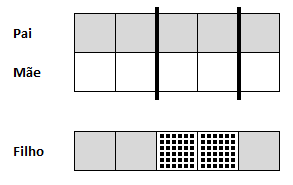
\includegraphics[width=.40\textwidth]{figs/materiais_metodo/software/pai-mae-filho-com-crossover.png} &
    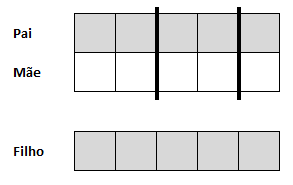
\includegraphics[width=.40\textwidth]{figs/materiais_metodo/software/pai-mae-filho-sem-crossover.png}
  \end{tabular}
  \caption{Diagrama do \emph{crossover} implementado. Na esquerda: \emph{crossover} acontece; na direita: \emph{crossover} acontece.}
	\label{fig:crossover_programa}
	\end{figure}

\vspace{1 cm}
\begin{lstlisting}
//============================================
void CrossOver2Pontos_serial(
  struct generation *g0,
  struct generation *g1,
  struct parametros *parametrosGA) {
//============================================

unsigned short int iIndividuo, idx_Pai, idx_Mae;
unsigned long int iGene;

struct individual *Pai, *Mae;
double f, p_aux;

for (iIndividuo = 0; iIndividuo < parametrosGA->numIndividuos; iIndividuo = iIndividuo + 1) {	

  idx_Pai = Randomico_int(0, parametrosGA->numIndividuos - 1);
  idx_Mae = Randomico_int(0, parametrosGA->numIndividuos - 1);

  Pai = &g0->individuo[idx_Pai];
  Mae = &g0->individuo[idx_Mae];

  p_aux = (double)((double)rand() / (double)RAND_MAX);

  f = -1.0F;

  g1->individuo[iIndividuo].pontos_de_corte[0] = Randomico_int(0, (parametrosGA->numGenes-1));
  g1->individuo[iIndividuo].pontos_de_corte[1] = Randomico_int(g1->individuo[iIndividuo].pontos_de_corte[0], (parametrosGA->numGenes-1));

  if (p_aux <= parametrosGA->probCrossOver) {

    f = (double)((double)rand()/(double)RAND_MAX);

    for (iGene = 0; iGene < g1->individuo[iIndividuo].pontos_de_corte[0]; iGene++) {
      g1->individuo[iIndividuo].gene[iGene] = Pai->gene[iGene];				
    }

    for (iGene = g1->individuo[iIndividuo].pontos_de_corte[0]; iGene < g1->individuo[iIndividuo].pontos_de_corte[1]; iGene++) {				
      g1->individuo[iIndividuo].gene[iGene] = f*Pai->gene[iGene] + (1 - f)*Mae->gene[iGene];				
    }

    for (iGene = g1->individuo[iIndividuo].pontos_de_corte[1]; iGene < parametrosGA->numGenes; iGene++) {
      g1->individuo[iIndividuo].gene[iGene] = Pai->gene[iGene];				
    }
  }
	
  else {
	
    for (iGene = 0; iGene < parametrosGA->numGenes; iGene++) {
      g1->individuo[iIndividuo].gene[iGene] =	g0->individuo[iIndividuo].gene[iGene];			
    }
  }
}
}
\end{lstlisting}
\vspace{1 cm}


%---------------------------------------------------
\subsection{Mutação}
%---------------------------------------------------

	Está no arquivo \textbf{\texttt{GA\_serial.h}}.
	
	Todos os genes de cada indivíduo estão sujeitos à mutação (laços das linhas 14 e 16). A condição de ocorrência é semelhante à do \emph{crossover}. Se uma probabilidade auxiliar, obtida aleatoriamente na linha 18, for menor que a problabilidade de mutação, o gene é alterado na linhas linhas 25--27 conforme equação \ref{eq:mutacao}. Os parâmetros necessários são obtidos nas linhas 21--23.
	
\vspace{1 cm}
\begin{lstlisting}
//============================================
void Mutacao_Serial(
  struct generation *geracao,
  struct parametros *parametrosGA) {
//============================================

unsigned short int iIndividuo;
unsigned long iGene;
unsigned short int L;
int termo_do_L;
double r, pAux;
double intensidadeMutacao = 10*geracao->Maior_fitness;

for (iIndividuo = 0; iIndividuo < parametrosGA->numIndividuos; iIndividuo++) {

  for (iGene = 0; iGene < parametrosGA->numGenes; iGene++) {

    pAux = (double)((double)rand() / (double)RAND_MAX);

    if (pAux <= parametrosGA->probMutacao) {
      L = Randomico_int(0, 10);
      r = (double)((double)rand() / (double)RAND_MAX) + 0.000002;
      termo_do_L = (int)pow((double)(-1),(int)L);
			
      geracao->individuo[iIndividuo].gene[iGene] =
          geracao->individuo[iIndividuo].gene[iGene] +
          (double)(termo_do_L * r * intensidadeMutacao);
    }
  }
}
}
\end{lstlisting}
\vspace{1 cm}


%---------------------------------------------------
\subsection{Fluxo principal}
%---------------------------------------------------
	
	Abaixo listo o código, presente no arquivo \textbf{\texttt{Serial\_novo.c}}, referente ao fluxo principal do GA (figura \ref{fig:fluxo}). Os operadores são aplicados na ordem: \emph{Fitness} (linha 7), Seleção (linha 44), \emph{Crossover} (linha 55) e Mutação (linha 66).
	
	O programa termina quando atinge o número máximo de gerações, testado na condição do \texttt{while} da linha 2, ou quando algum dos critérios de parada de precisão é atingido (linhas 37--40), definidos pelas equações \ref{eq:criterioParada024} e \ref{eq:criterioParada13}. Note que elas são testados logo após o \emph{fitness}, afinal, se uma geração contém boas soluções, não deve ser alterada pelos outros operadores genéticos.

\vspace{1 cm}
\begin{lstlisting}
//============================================
while (iGeracao < parmsPrograma.parmQtdeMaxGeracoes) {

  // FITNESS
  time_i = clock();
	
  Fitness_Serial(
    parmTipoFitnessEquacao,
    TipoCalculoGradRho,
    geracao0,
    &parametrosGA,
    &parametrosMetodo,
    Hamiltoniano,
    parametrosGA.numGenes,
    parametrosMetodo.lambda,
    parametrosMetodo.rho_minimo,
    MatrizIdentidade
  );
	
  time_f = clock();

  if (flagImprimeTempo == 1) {
    imprimeTempo(
      1, 0, 0, iGeracao, 4, 2, time_i, time_f,
      &parametrosGA, &parametrosMetodo, &parmsPrograma
    );
  }

  if (flagImprimeComportamentoFitness == 1) {
    imprimeComportamentoFitness(
      1, codMaquina, tipoPrograma, 0, iGeracao, geracao0,
      &parametrosMetodo, &parametrosGA, &parmsPrograma
    );
  }

  // CRITERIOS DE PARADA
  flagAtingiuTolerancia = atingiuCriterioDeParada(parmTipoFitnessEquacao, tolerancia, geracao0);
	
  if (flagAtingiuTolerancia == 1)
    break;

  // SELECAO
  time_i = clock();
  Selecao_Por_Torneio_serial(geracao0, geracao1, &parametrosGA);
  time_f = clock();
  if (flagImprimeTempo == 1) {
    imprimeTempo(
      1, 0, 0, iGeracao, 5, 2, time_i, time_f,
      &parametrosGA, &parametrosMetodo, &parmsPrograma
    );
  }

  // CROSSOVER
  time_i = clock();
  CrossOver2Pontos_serial(geracao1, geracao0, &parametrosGA);
  time_f = clock();
  if (flagImprimeTempo == 1) {
    imprimeTempo(
      1, 0, 0, iGeracao, 6, 2, time_i, time_f,
      &parametrosGA, &parametrosMetodo, &parmsPrograma
    );
}

  // MUTACAO
  time_i = clock();
  Mutacao_Serial(geracao0, &parametrosGA);
  time_f = clock();
  if (flagImprimeTempo == 1) {
    imprimeTempo(
      1, 0, 0, iGeracao, 7, 2, time_i, time_f,
      &parametrosGA, &parametrosMetodo, &parmsPrograma
    );
  }

  iGeracao++;
}
\end{lstlisting}
\vspace{1 cm}	